% Supplementary material for:
% "Feature Subsampling in Hybrid Wi-Fi RTT--RSS Fingerprinting:
%  Radio-Map Density, Ratio Selection, and Calibration With Clustered Scans"
% Compile from this directory:  pdflatex supplementary_material.tex
\documentclass[10pt]{article}
\usepackage[margin=2cm]{geometry}
\usepackage{amsmath,amssymb}
\usepackage{booktabs}
\usepackage{graphicx}
\usepackage[hidelinks]{hyperref}
\graphicspath{{../figures/results/}}
\renewcommand{\thetable}{S\arabic{table}}
\renewcommand{\thefigure}{S\arabic{figure}}

\title{Supplementary Material\\ \large Feature Subsampling in Hybrid Wi-Fi RTT--RSS Fingerprinting: Radio-Map Density, Ratio Selection, and Calibration With Clustered Scans}
\author{Nabil Abdelkader Nouri and Salim Naouri}
\date{}

\begin{document}
\maketitle

This document collects material that supports the main paper but is not needed to follow its argument: the evidence for the EETAC acquisition-day frame alignment, the effect of the alignment on all EETAC protocols, the EETAC ratio sweep, the density sweep with its spread over random RP subsets, screening experiments that were not retained, the computational cost of the 300-tree models, single-split uncertainty regions with covariance-aware ellipses, and figures that were moved from the main paper to shorten it. All tables are generated from the released experiment outputs by \texttt{scripts/extensions/make\_supplementary.py}.

\section{EETAC Acquisition-Day Frame Alignment}

Table~\ref{tab:s_frame_audit} gives the evidence for the mirrored coordinate frame of the second EETAC acquisition day, and Table~\ref{tab:s_alignment} shows its effect. Without alignment, the RP-grouped and cross-day errors exceed 4~m; after alignment, cross-day errors are 1.2--1.7~m. In both cases $\rho=0.7$ is better than $\rho=1$.

\section{EETAC Ratio Sweep and Density Sweep}

Table~\ref{tab:s_eetac_ratio} reports the EETAC sweep summarized in the ratio-selection subsection of the paper, and Table~\ref{tab:s_density} gives the numerical values behind the density figure, including the standard deviation over ten random RP subsets.

\section{Screening Experiments}

Table~\ref{tab:s_screening} reports variants of the point predictor that were screened but not retained: per-tree random subspaces~\cite{ho1998random}, AP-level subspaces that keep each AP's RTT and RSS together, RTT multilateration features computed from the published AP coordinates, and a residual model that corrects a multilateration estimate. Table~\ref{tab:s_local} reports locally adaptive conformal regions that normalize the residual by the spread of the tree predictions.

\section{Computational Cost and Single-Split Uncertainty Regions}

Table~\ref{tab:s_efficiency} reports training time, inference time, and serialized size of the two 300-tree models. Table~\ref{tab:s_uncertainty} reports circular and covariance-aware elliptical regions for one calibration split (seed 42); their variability over repeated splits, and the comparison with group calibration, are given in the calibration table of the paper.

\section{Tables Moved from the Main Paper}

Table~\ref{tab:cross_day} gives the seed-42 cross-day results with all metrics, Table~\ref{tab:data_utilization} the cost of reserving calibration RPs for the point predictor, and Table~\ref{tab:compact_models} the values behind the model-size figure of the paper.

\section{Additional Figures}

Figures~\ref{fig:s_error_cdf}--\ref{fig:s_ratio_selection} were moved from the main paper to shorten it; Figs.~\ref{fig:s_original_accuracy}--\ref{fig:s_uncertainty_area} duplicate information given in tables.

% Generated by scripts/extensions/make_supplementary.py -- do not edit by hand.

\begin{table}[!ht]
\centering
\caption{EETAC acquisition-day frame audit. For each of the 25 Day~1 RPs, the Day~2 RP with the nearest median Google-AP RTT fingerprint is found; the table counts how often it lies at the position predicted by each coordinate mapping. Selected mapping: mirror y.}
\label{tab:s_frame_audit}
\footnotesize
\begin{tabular}{lc}
\toprule
Mapping of Day~2 coordinates & Matching RPs (of 25) \\
\midrule
Identity ($y\mapsto y$) & 4 \\
Mirror ($y\mapsto 8-y$) & 22 \\
Uninformative (central row $y=4$~m) & 5 \\
\bottomrule
\end{tabular}
\end{table}

\begin{table}[!ht]
\centering
\caption{EETAC 2D RMSE (m) with and without acquisition-day frame alignment, mean of three seeds (0--2). Without alignment, pooled and cross-day experiments mix two physical locations under one label.}
\label{tab:s_alignment}
\footnotesize
\begin{tabular}{lllcccc}
\toprule
Frames & Scenario & $\rho$ & Sample CV & RP-grouped CV & D1$\rightarrow$D2 & D2$\rightarrow$D1 \\
\midrule
not aligned & Medium (4 APs) & 1.0 & 0.618 & 4.874 & 5.328 & 5.487 \\
not aligned & Medium (4 APs) & 0.7 & 0.522 & 4.738 & 5.263 & 5.414 \\
not aligned & High (7 APs) & 1.0 & 0.593 & 4.330 & 5.336 & 5.493 \\
not aligned & High (7 APs) & 0.7 & 0.466 & 4.129 & 5.171 & 5.394 \\
\midrule
aligned & Medium (4 APs) & 1.0 & 0.366 & 2.906 & 1.341 & 1.593 \\
aligned & Medium (4 APs) & 0.7 & 0.314 & 2.497 & 1.254 & 1.259 \\
aligned & High (7 APs) & 1.0 & 0.365 & 2.895 & 1.376 & 1.714 \\
aligned & High (7 APs) & 0.7 & 0.312 & 2.514 & 1.336 & 1.489 \\
\bottomrule
\end{tabular}
\end{table}

\begin{table}[!ht]
\centering
\caption{EETAC ratio sweep (frame-aligned), 2D RMSE (m), mean of three seeds. Best ratio per column in bold.}
\label{tab:s_eetac_ratio}
\footnotesize
\begin{tabular}{lccccc}
\toprule
Scenario & $\rho$ & Sample CV & RP-grouped CV & D1$\rightarrow$D2 & D2$\rightarrow$D1 \\
\midrule
Medium (4 APs) & 0.20 & 0.331 & 2.729 & 1.647 & 1.621 \\
 & 0.35 & \textbf{0.292} & 2.471 & 1.285 & 1.330 \\
 & 0.50 & 0.301 & \textbf{2.434} & \textbf{1.237} & \textbf{1.234} \\
 & 0.70 & 0.314 & 2.497 & 1.254 & 1.259 \\
 & 0.85 & 0.325 & 2.605 & 1.275 & 1.367 \\
 & 1.00 & 0.366 & 2.906 & 1.341 & 1.593 \\
\midrule
High (7 APs) & 0.20 & 0.299 & 2.587 & 3.186 & 2.838 \\
 & 0.35 & \textbf{0.286} & 2.445 & 2.203 & 2.024 \\
 & 0.50 & 0.304 & \textbf{2.435} & 1.468 & 1.506 \\
 & 0.70 & 0.312 & 2.514 & 1.336 & \textbf{1.489} \\
 & 0.85 & 0.331 & 2.635 & \textbf{1.322} & 1.523 \\
 & 1.00 & 0.365 & 2.895 & 1.376 & 1.714 \\
\bottomrule
\end{tabular}
\end{table}

\begin{table*}[!ht]
\centering
\caption{Official-test paper-compatible error (m, mean $\pm$ std over 10 random RP subsets) versus subspace ratio for thinned training radio maps (fraction and number of training RPs). Best ratio in bold.}
\label{tab:s_density}
\scriptsize
\setlength{\tabcolsep}{3pt}
\begin{tabular}{llcccccc}
\toprule
Dataset & Map & $\rho=0.2$ & $\rho=0.35$ & $\rho=0.5$ & $\rho=0.7$ & $\rho=0.85$ & $\rho=1.0$ \\
\midrule
Building & 100\% (483) & 0.530$\pm$0.005 & 0.508$\pm$0.003 & \textbf{0.505$\pm$0.004} & 0.518$\pm$0.004 & 0.543$\pm$0.004 & 0.605$\pm$0.005 \\
 & 75\% (362) & 0.580$\pm$0.010 & \textbf{0.566$\pm$0.014} & 0.568$\pm$0.013 & 0.590$\pm$0.017 & 0.627$\pm$0.022 & 0.705$\pm$0.044 \\
 & 50\% (242) & 0.682$\pm$0.028 & \textbf{0.670$\pm$0.028} & 0.685$\pm$0.028 & 0.728$\pm$0.035 & 0.789$\pm$0.043 & 0.899$\pm$0.070 \\
 & 25\% (121) & \textbf{0.916$\pm$0.043} & 0.925$\pm$0.058 & 0.953$\pm$0.070 & 0.998$\pm$0.076 & 1.074$\pm$0.092 & 1.198$\pm$0.127 \\
\midrule
Apartment & 100\% (81) & 0.710$\pm$0.008 & 0.647$\pm$0.008 & 0.585$\pm$0.008 & 0.567$\pm$0.007 & \textbf{0.562$\pm$0.003} & 0.598$\pm$0.002 \\
 & 75\% (61) & 0.743$\pm$0.027 & 0.680$\pm$0.027 & 0.625$\pm$0.028 & 0.616$\pm$0.032 & \textbf{0.613$\pm$0.030} & 0.653$\pm$0.058 \\
 & 50\% (40) & 0.831$\pm$0.055 & 0.785$\pm$0.065 & \textbf{0.767$\pm$0.089} & 0.771$\pm$0.104 & 0.793$\pm$0.127 & 0.885$\pm$0.155 \\
 & 25\% (20) & 0.973$\pm$0.056 & \textbf{0.938$\pm$0.057} & 0.950$\pm$0.053 & 0.980$\pm$0.063 & 1.024$\pm$0.075 & 1.144$\pm$0.144 \\
\midrule
Office & 100\% (28) & 0.407$\pm$0.006 & 0.353$\pm$0.004 & 0.341$\pm$0.003 & \textbf{0.338$\pm$0.003} & 0.346$\pm$0.003 & 0.373$\pm$0.004 \\
 & 75\% (21) & 0.446$\pm$0.023 & 0.412$\pm$0.037 & 0.394$\pm$0.042 & \textbf{0.392$\pm$0.045} & 0.397$\pm$0.056 & 0.417$\pm$0.075 \\
 & 50\% (14) & 0.501$\pm$0.037 & \textbf{0.487$\pm$0.046} & 0.487$\pm$0.057 & 0.496$\pm$0.068 & 0.510$\pm$0.081 & 0.535$\pm$0.094 \\
 & 25\% (7) & 0.638$\pm$0.098 & \textbf{0.625$\pm$0.100} & 0.625$\pm$0.100 & 0.640$\pm$0.112 & 0.664$\pm$0.111 & 0.694$\pm$0.121 \\
\bottomrule
\end{tabular}
\end{table*}

\begin{table*}[!ht]
\centering
\caption{Screening experiments not retained in the main paper (paper-compatible metric in m, official test / pooled RP-grouped CV; Office and Apartment: mean of three seeds, Building: one seed). Per-tree subspaces are worse than per-split subsampling with or without pairing an AP's RTT and RSS. Geometry features from RTT multilateration with the published AP coordinates help the small three- and four-AP environments under RP-grouped CV but not Building; the residual variant is unstable because multilateration diverges for some scans.}
\label{tab:s_screening}
\footnotesize
\begin{tabular}{lccc}
\toprule
Variant & Building & Apartment & Office \\
\midrule
Per-split subsampling, $\rho=0.7$ (reference) & 0.526 / 0.707 & 0.564 / 0.617 & 0.339 / 0.464 \\
Per-tree feature subspace, $70\%$ of features & 0.540 / 0.721 & 0.645 / 0.649 & 0.364 / 0.467 \\
Per-tree AP subspace, $70\%$ of APs (RTT+RSS kept together) & 0.552 / 0.731 & 0.648 / 0.701 & 0.352 / 0.485 \\
Per-tree AP subspace, $50\%$ of APs & 0.620 / 0.743 & 0.841 / 0.822 & 0.352 / 0.485 \\
\midrule
RF $\rho=0.7$, RTT+RSS only (reference) & 0.526 / 0.707 & 0.564 / 0.617 & 0.339 / 0.464 \\
+ multilateration features (position, \#APs, residual) & 0.510 / 0.713 & 0.529 / 0.594 & 0.343 / 0.396 \\
+ multilateration + RTT/RSS differences to strongest AP & 0.518 / 0.703 & 0.496 / 0.623 & 0.530 / 0.413 \\
Multilateration + RF residual correction & 0.577 / 0.720 & 0.570 / 7.573 & 0.279 / 0.487 \\
\bottomrule
\end{tabular}
\end{table*}

\begin{table*}[!ht]
\centering
\caption{Screening of locally adaptive conformal regions (scan-level split conformal; coverage / mean area in m$^2$). Local regions normalize the residual by the spread of the 300 tree predictions (plus a fixed floor equal to the median spread). Mean over three seeds (Building: one).}
\label{tab:s_local}
\footnotesize
\begin{tabular}{llcccc}
\toprule
Dataset & $1-\alpha$ & Global circle & Global ellipse & Local circle & Local ellipse \\
\midrule
Building & 90\% & 0.936 / 5.57 & 0.938 / 5.64 & 0.961 / 6.55 & 0.958 / 6.35 \\
 & 95\% & 0.962 / 7.61 & 0.959 / 7.23 & 0.976 / 7.69 & 0.973 / 7.56 \\
Apartment & 90\% & 0.911 / 7.44 & 0.905 / 7.10 & 0.929 / 6.85 & 0.912 / 5.56 \\
 & 95\% & 0.953 / 9.99 & 0.945 / 8.40 & 0.979 / 10.19 & 0.984 / 8.43 \\
Office & 90\% & 0.856 / 2.07 & 0.826 / 1.92 & 0.818 / 1.90 & 0.853 / 1.94 \\
 & 95\% & 0.887 / 2.36 & 0.851 / 2.18 & 0.876 / 2.20 & 0.893 / 2.15 \\
\bottomrule
\end{tabular}
\end{table*}

\begin{table*}[!ht]
\centering
\caption{Accuracy and cost of the 300-tree models (seed 42, 20 threads). Error: paper-compatible metric for the original benchmark, 2D RMSE (sample-level CV) for EETAC. Wall-clock times depend on system load; compact forests are analyzed in the paper.}
\label{tab:s_efficiency}
\footnotesize
\begin{tabular}{lcccccccc}
\toprule
 & \multicolumn{2}{c}{Error (m)} & \multicolumn{2}{c}{Train (s)} & \multicolumn{2}{c}{Inference ($\mu$s/scan)} & \multicolumn{2}{c}{Size (MB)} \\
Dataset & $\rho=1$ & $\rho=0.7$ & $\rho=1$ & $\rho=0.7$ & $\rho=1$ & $\rho=0.7$ & $\rho=1$ & $\rho=0.7$ \\
\midrule
Building & 0.599 & 0.513 & 13.63 & 6.35 & 12.93 & 9.29 & 58.88 & 64.26 \\
Office & 0.370 & 0.343 & 0.56 & 0.40 & 67.62 & 67.21 & 2.86 & 3.41 \\
Apartment & 0.600 & 0.569 & 0.80 & 0.74 & 31.30 & 38.30 & 13.32 & 14.85 \\
EETAC Medium (4 APs) & 0.331 & 0.292 & 0.56 & 0.49 & -- & -- & -- & -- \\
EETAC High (7 APs) & 0.329 & 0.292 & 0.61 & 0.52 & -- & -- & -- & -- \\
\bottomrule
\end{tabular}
\end{table*}

\begin{table*}[!ht]
\centering
\caption{Circular and covariance-aware elliptical regions in a single calibration split (seed 42): empirical coverage (Cov.) and area (m$^2$). $G$: number of calibration RPs. RP-count: the conservative level computed with $n=G$. The variability over calibration splits, and the valid group-conformal rule, are reported in the paper.}
\label{tab:s_uncertainty}
\footnotesize
\setlength{\tabcolsep}{3.5pt}
\begin{tabular}{llcccccccc}
\toprule
 & & \multicolumn{4}{c}{$1-\alpha=0.90$} & \multicolumn{4}{c}{$1-\alpha=0.95$} \\
 & & \multicolumn{2}{c}{Circle} & \multicolumn{2}{c}{Ellipse} & \multicolumn{2}{c}{Circle} & \multicolumn{2}{c}{Ellipse} \\
Dataset & Calibration & Cov. & Area & Cov. & Area & Cov. & Area & Cov. & Area \\
\midrule
Building ($G=121$) & Split conformal, scan-level & 0.952 & 8.21 & 0.954 & 7.90 & 0.984 & 16.71 & 0.985 & 15.92 \\
 & Split conformal, RP-count & 0.963 & 9.23 & 0.960 & 8.55 & 0.988 & 20.25 & 0.989 & 19.63 \\
 & Grouped-OOF empirical & 0.965 & 5.69 & 0.965 & 5.32 & 0.983 & 9.28 & 0.989 & 8.66 \\
\midrule
Office ($G=7$) & Split conformal, scan-level & 0.999 & 3.28 & 0.965 & 3.14 & 0.999 & 3.83 & 0.982 & 3.55 \\
 & Split conformal, RP-count & 1.000 & 14.46 & 1.000 & 14.40 & 1.000 & 14.46 & 1.000 & 14.40 \\
 & Grouped-OOF empirical & 0.982 & 2.66 & 0.943 & 2.50 & 0.999 & 6.13 & 0.999 & 5.44 \\
\midrule
Apartment ($G=21$) & Split conformal, scan-level & 0.828 & 6.39 & 0.822 & 5.89 & 0.949 & 9.93 & 0.918 & 9.51 \\
 & Split conformal, RP-count & 0.954 & 10.22 & 0.923 & 9.70 & 0.997 & 15.87 & 0.997 & 17.31 \\
 & Grouped-OOF empirical & 0.920 & 6.07 & 0.901 & 5.28 & 0.942 & 8.45 & 0.935 & 7.49 \\
\bottomrule
\end{tabular}
\end{table*}

\begin{table*}[!t]
\centering
\caption{Cross-day EETAC temporal generalization after acquisition-day frame alignment (seed 42). Each model is trained on all scans of one day and tested on all scans of the other. Negative improvements indicate that F0.7 is worse.}
\label{tab:cross_day}
\footnotesize
\setlength{\tabcolsep}{5pt}
\begin{tabular}{llcccccc}
\toprule
 & & \multicolumn{3}{c}{2D RMSE (m)} & \multicolumn{3}{c}{$P_{90}$ (m)} \\
\cmidrule(lr){3-5}\cmidrule(lr){6-8}
Scenario & Direction & F1.0 & F0.7 & Impr. (\%) & F1.0 & F0.7 & Impr. (\%) \\
\midrule
Medium (4 APs) & Day~1$\rightarrow$Day~2 & 1.331 & \textbf{1.253} & 5.89 & 2.105 & \textbf{2.060} & 2.13 \\
 & Day~2$\rightarrow$Day~1 & 1.541 & \textbf{1.222} & 20.68 & 2.665 & \textbf{2.244} & 15.78 \\
\midrule
High (7 APs) & Day~1$\rightarrow$Day~2 & \textbf{1.378} & 1.394 & -1.16 & \textbf{2.169} & 2.331 & -7.46 \\
 & Day~2$\rightarrow$Day~1 & 1.674 & \textbf{1.465} & 12.52 & 2.902 & \textbf{2.641} & 9.01 \\
\bottomrule
\end{tabular}
\end{table*}

\begin{table}[!t]
\centering
\caption{Effect of training the proposed predictor on the grouped fitting subset versus all official training reference points (paper-compatible metric).}
\label{tab:data_utilization}
\footnotesize
\setlength{\tabcolsep}{5pt}
\begin{tabular}{lccccc}
\toprule
 & \multicolumn{2}{c}{Training RPs} & \multicolumn{2}{c}{Error (m)} & \\
\cmidrule(lr){2-3}\cmidrule(lr){4-5}
Dataset & Subset & 100\% & Subset & 100\% & Impr. (\%) \\
\midrule
Building  & 362 & 483 & 0.594 & \textbf{0.513} & 13.59 \\
Office    & 21  & 28  & 0.345 & \textbf{0.343} & 0.38 \\
Apartment & 60  & 81  & 0.645 & \textbf{0.569} & 11.70 \\
\bottomrule
\end{tabular}
\end{table}

\begin{table*}[!t]
\centering
\caption{Compact forests. Serialized model size (Python pickle), single-thread inference time per scan, training time (20 threads, Intel Core i5-13500HX), and official-test accuracy. Error: paper-compatible metric (m); RMSE: true 2D RMSE (m).}
\label{tab:compact_models}
\footnotesize
\setlength{\tabcolsep}{4pt}
\begin{tabular}{lcccccccc}
\toprule
Dataset & $\rho$ & Trees & Min. leaf & Size (MB) & Inference ($\mu$s/scan) & Train (s) & Error (m) & 2D RMSE (m) \\
\midrule
Building & 1.0 & 300 & 1 & 58.79 & 13.2 & 9.92 & 0.605 & 0.859 \\
 & 0.7 & 300 & 1 & 64.31 & 27.7 & 13.35 & 0.526 & 0.751 \\
 & 0.7 & 100 & 1 & 21.45 & 5.6 & 3.12 & 0.526 & 0.750 \\
 & 0.7 & 50 & 1 & 10.71 & 2.2 & 1.10 & 0.536 & 0.764 \\
 & 0.7 & 50 & 5 & 8.49 & 1.8 & 1.12 & 0.548 & 0.782 \\
\midrule
Apartment & 1.0 & 300 & 1 & 13.31 & 36.7 & 1.73 & 0.597 & 0.863 \\
 & 0.7 & 300 & 1 & 14.96 & 61.4 & 1.25 & 0.561 & 0.807 \\
 & 0.7 & 100 & 1 & 4.98 & 14.4 & 0.49 & 0.555 & 0.798 \\
 & 0.7 & 50 & 1 & 2.49 & 8.5 & 0.28 & 0.566 & 0.815 \\
 & 0.7 & 50 & 5 & 1.93 & 5.2 & 0.23 & 0.595 & 0.862 \\
\midrule
Office & 1.0 & 300 & 1 & 2.85 & 67.4 & 0.80 & 0.377 & 0.533 \\
 & 0.7 & 300 & 1 & 3.40 & 77.8 & 0.84 & 0.338 & 0.478 \\
 & 0.7 & 100 & 1 & 1.13 & 19.6 & 0.30 & 0.338 & 0.478 \\
 & 0.7 & 50 & 1 & 0.56 & 10.4 & 0.17 & 0.342 & 0.484 \\
 & 0.7 & 50 & 5 & 0.51 & 14.0 & 0.19 & 0.352 & 0.497 \\
\bottomrule
\end{tabular}
\end{table*}

\clearpage
% Figures moved from the main paper to shorten it; regenerated by run_all_paper_experiments.py.

\begin{figure}[!ht]
	\centering
	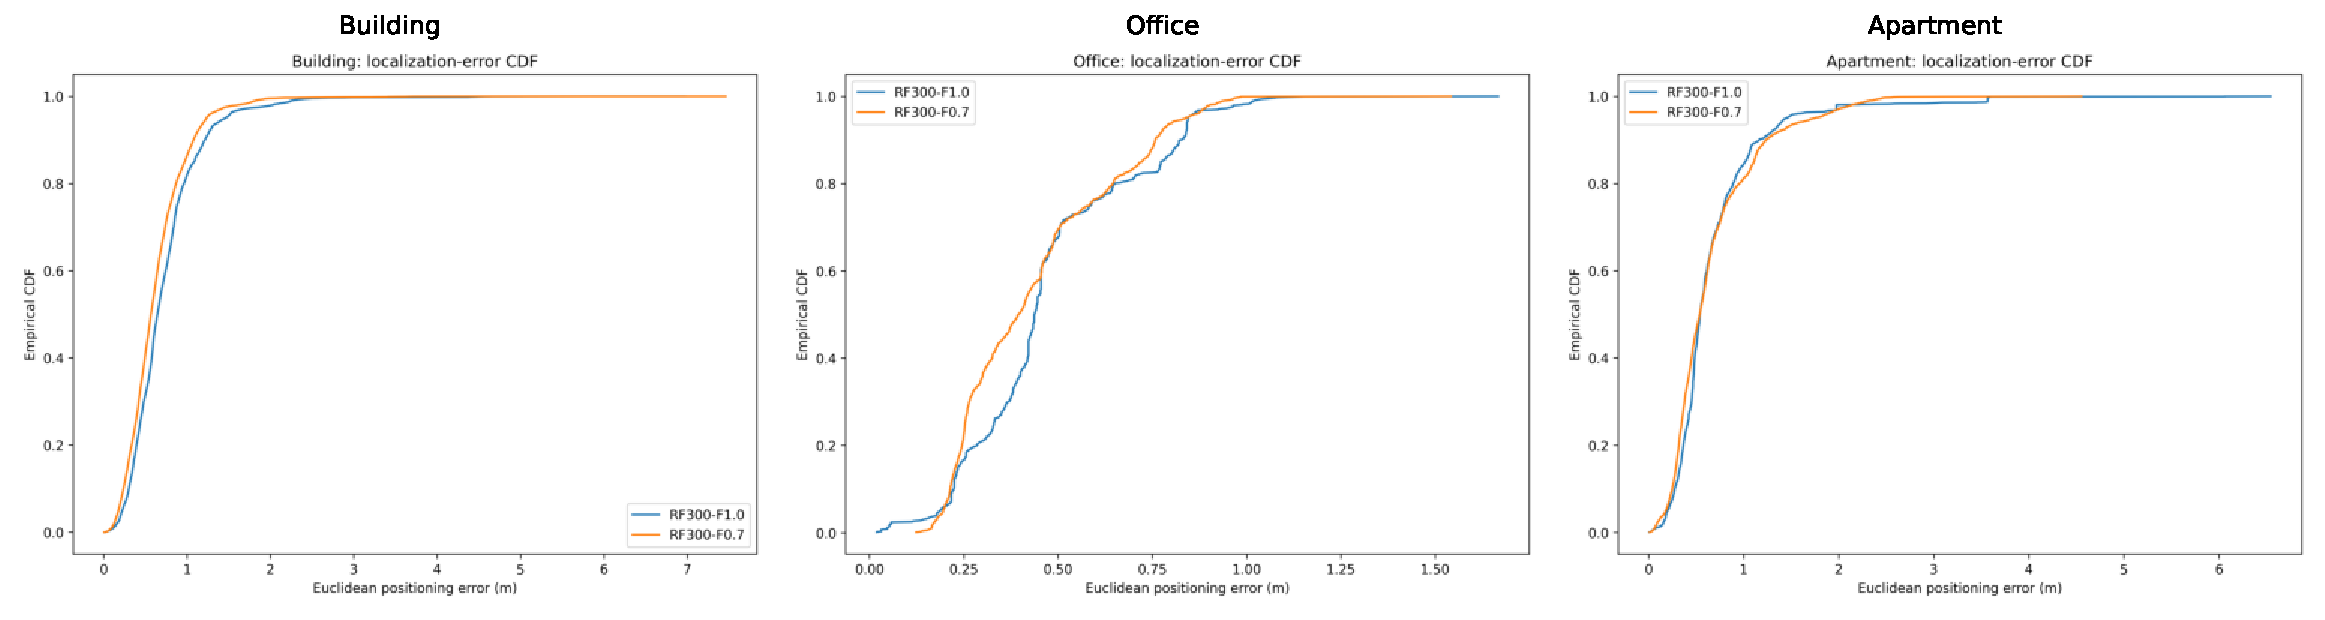
\includegraphics[width=\textwidth]{fig07_error_cdf.pdf}
	\caption{Empirical cumulative distributions of the positioning error of RF300-F1.0 and RF300-F0.7 on the official Building, Office, and Apartment test sets.}
	\label{fig:s_error_cdf}
\end{figure}

\begin{figure}[!ht]
	\centering
	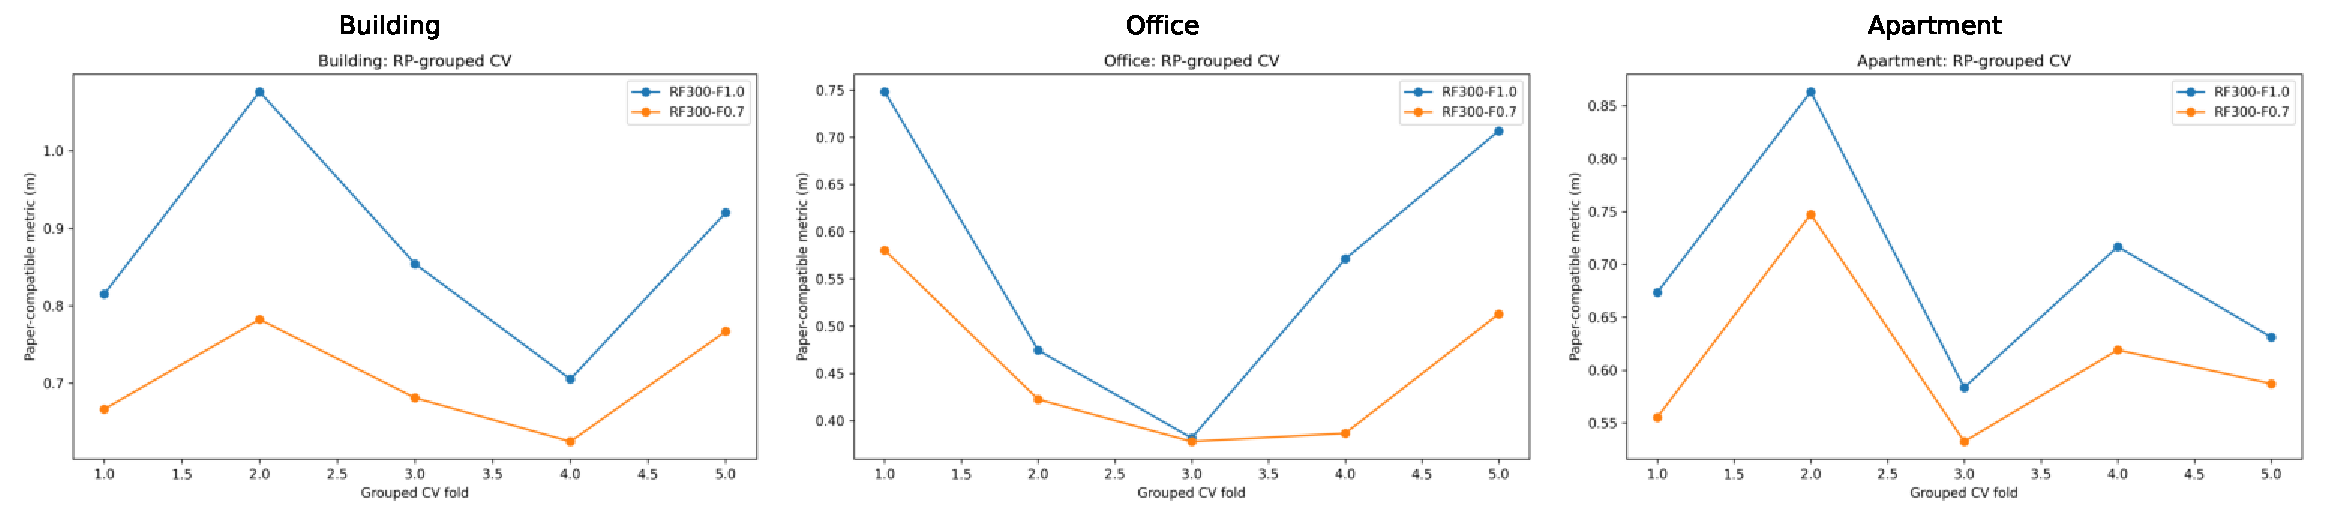
\includegraphics[width=\textwidth]{fig08_grouped_cv.pdf}
	\caption{Fold-level results of five-fold RP-grouped validation on the original benchmark (pooled values in the RP-grouped cross-validation table of the paper).}
	\label{fig:s_grouped_cv}
\end{figure}

\begin{figure}[!ht]
	\centering
	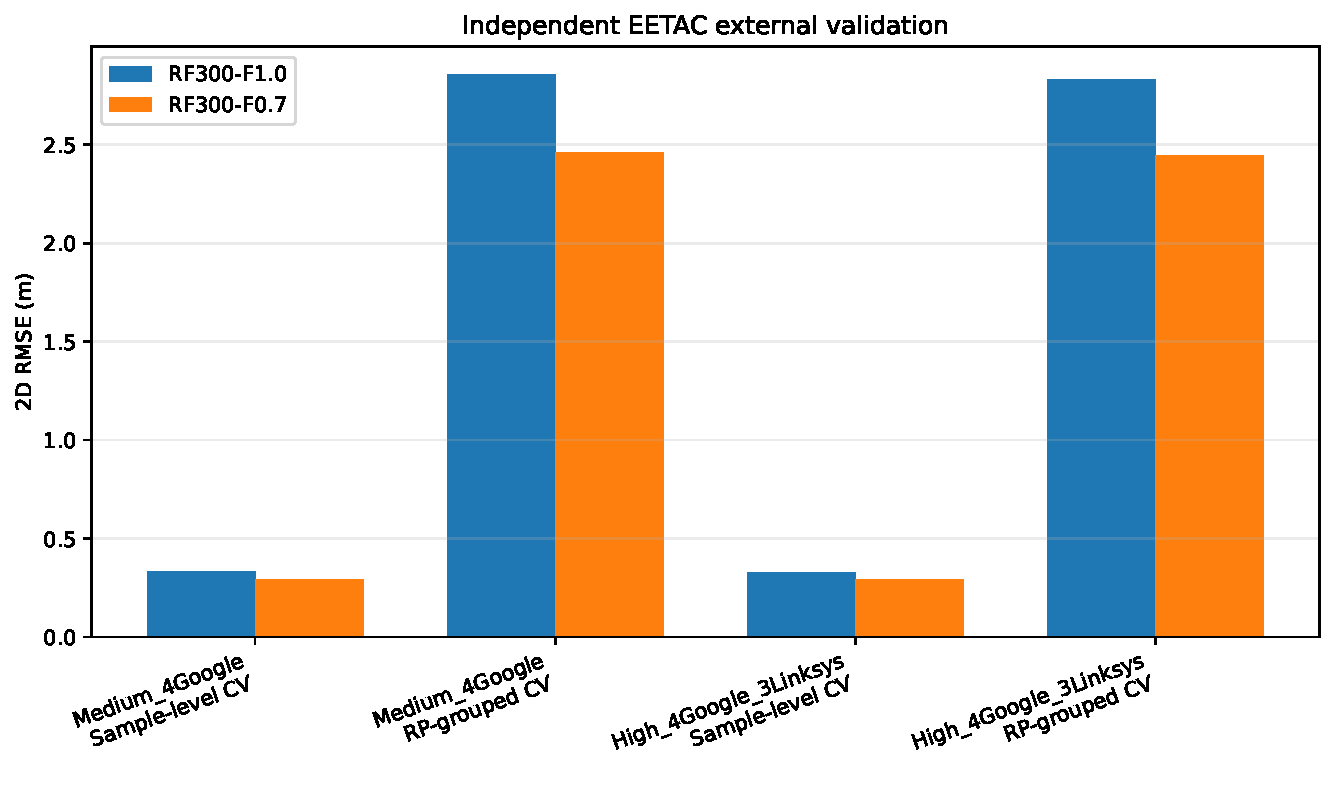
\includegraphics[width=0.8\textwidth]{fig09_eetac_external_validation.pdf}
	\caption{External validation on the EETAC auditorium dataset (frame-aligned, seed 42) using sample-level and RP-grouped protocols.}
	\label{fig:s_eetac}
\end{figure}

\begin{figure}[!ht]
	\centering
	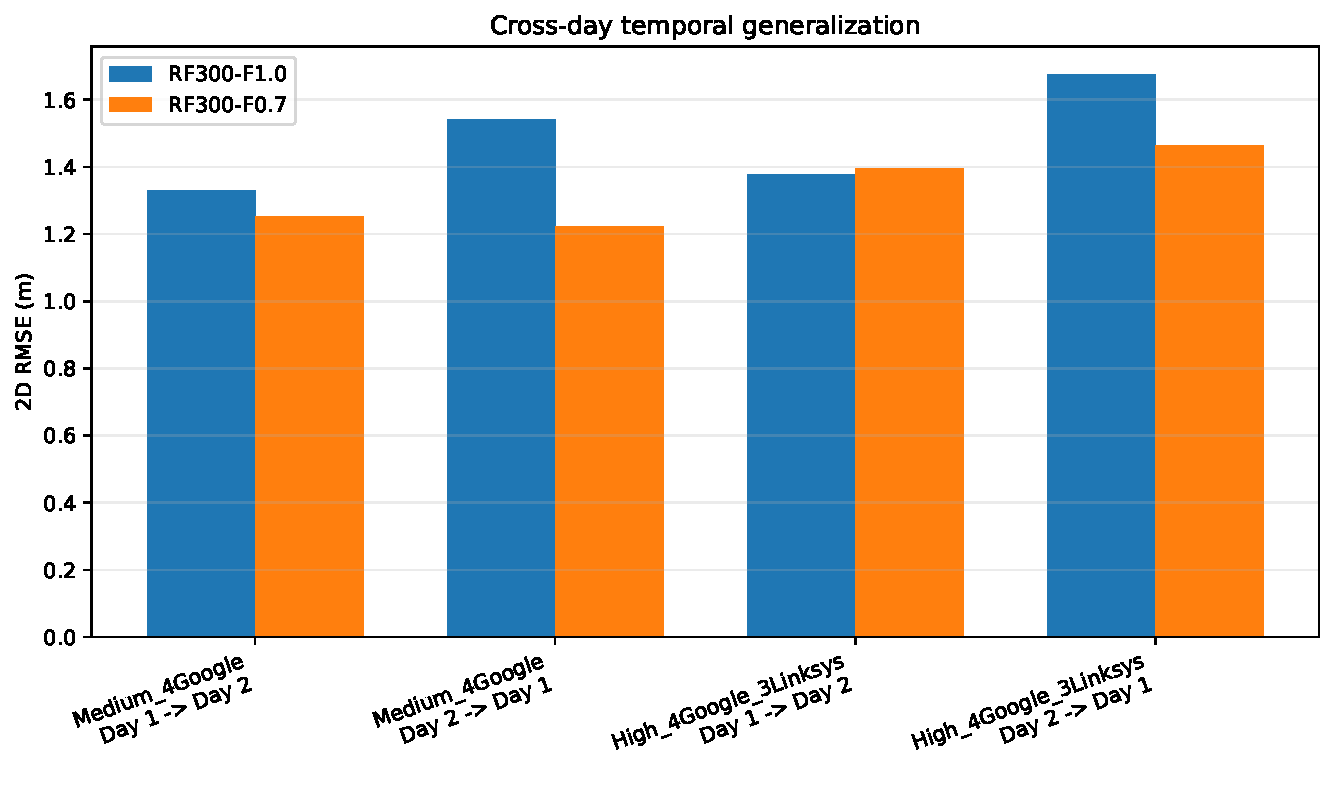
\includegraphics[width=0.8\textwidth]{fig11_cross_day.pdf}
	\caption{Cross-day EETAC results after frame alignment (seed 42). Each model is trained on one acquisition day and evaluated on the other.}
	\label{fig:s_cross_day}
\end{figure}

\begin{figure}[!ht]
	\centering
	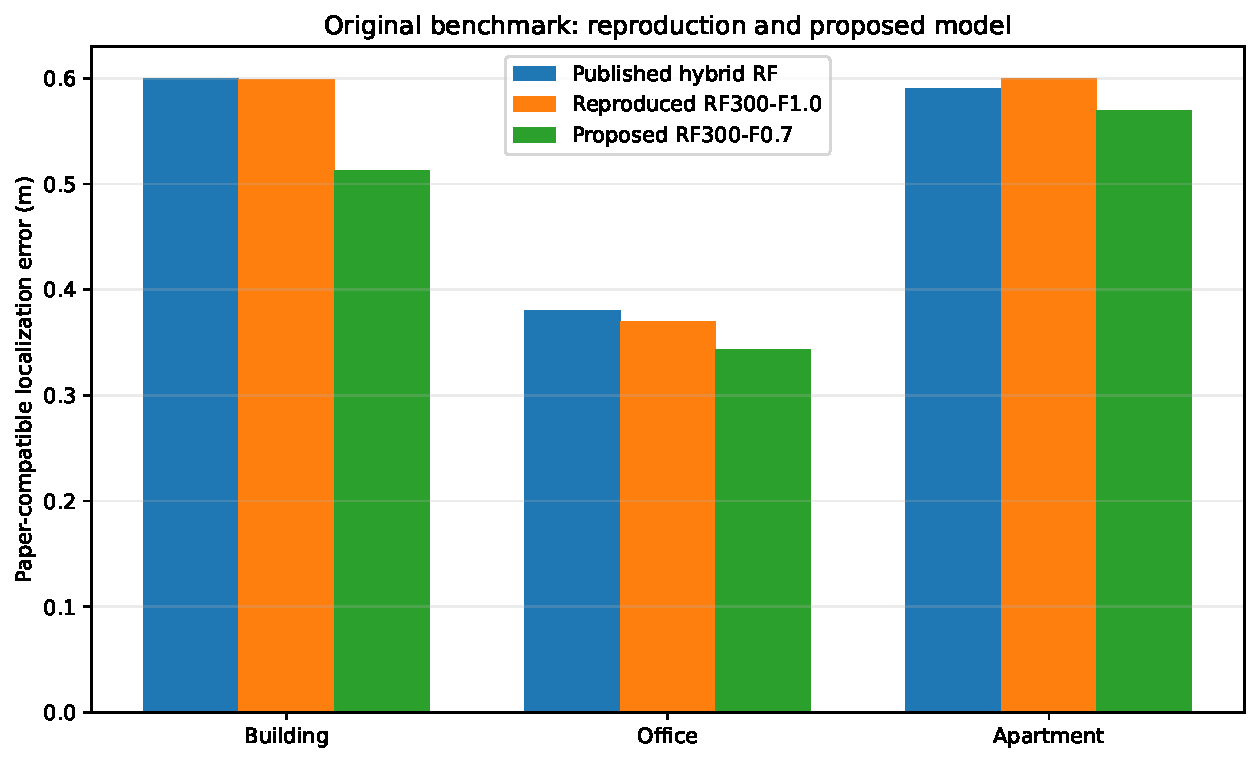
\includegraphics[width=0.8\textwidth]{fig06_original_accuracy.pdf}
	\caption{Paper-compatible error on the original benchmark: published hybrid RF, reproduced RF300-F1.0, and RF300-F0.7 (official RP-disjoint test sets).}
	\label{fig:s_original_accuracy}
\end{figure}

\begin{figure}[!ht]
	\centering
	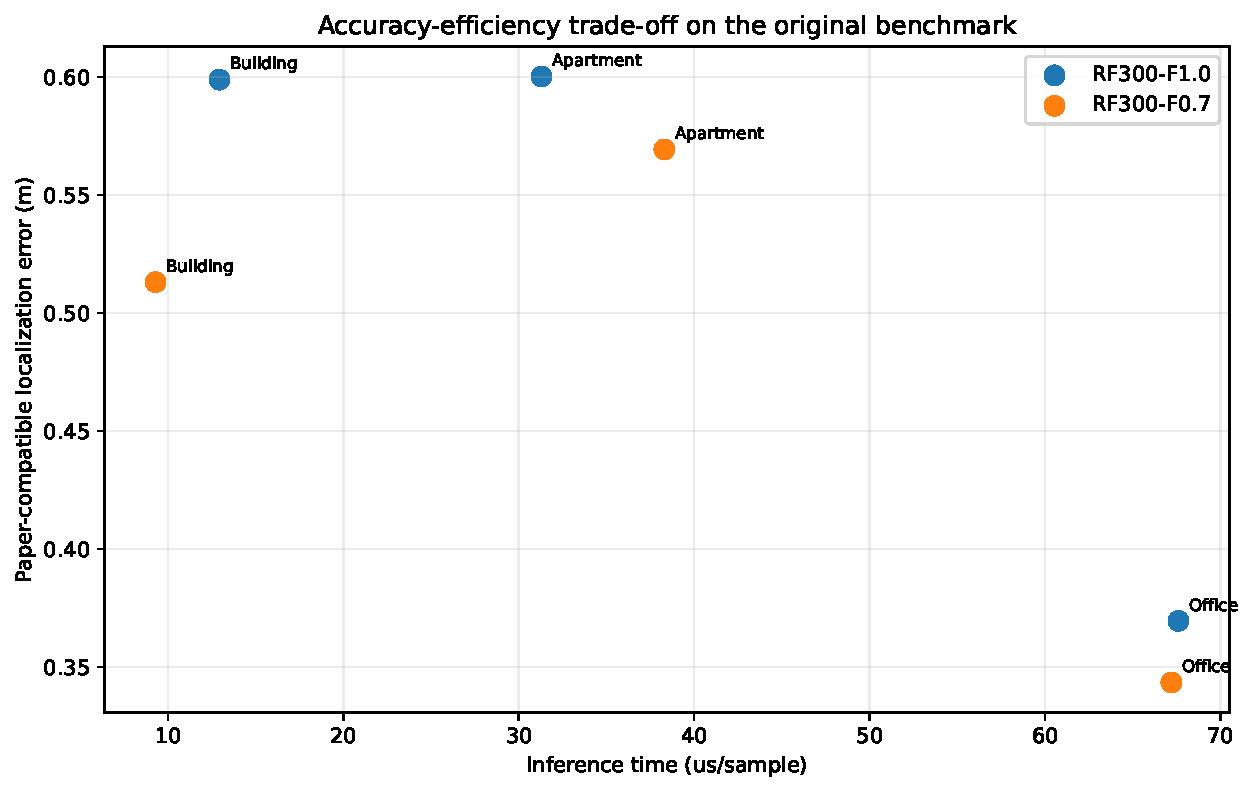
\includegraphics[width=0.8\textwidth]{fig10_accuracy_efficiency.pdf}
	\caption{Accuracy versus inference time of the 300-tree RF300-F1.0 and RF300-F0.7 models (values in Table~\ref{tab:s_efficiency}).}
	\label{fig:s_accuracy_efficiency}
\end{figure}

\begin{figure}[!ht]
	\centering
	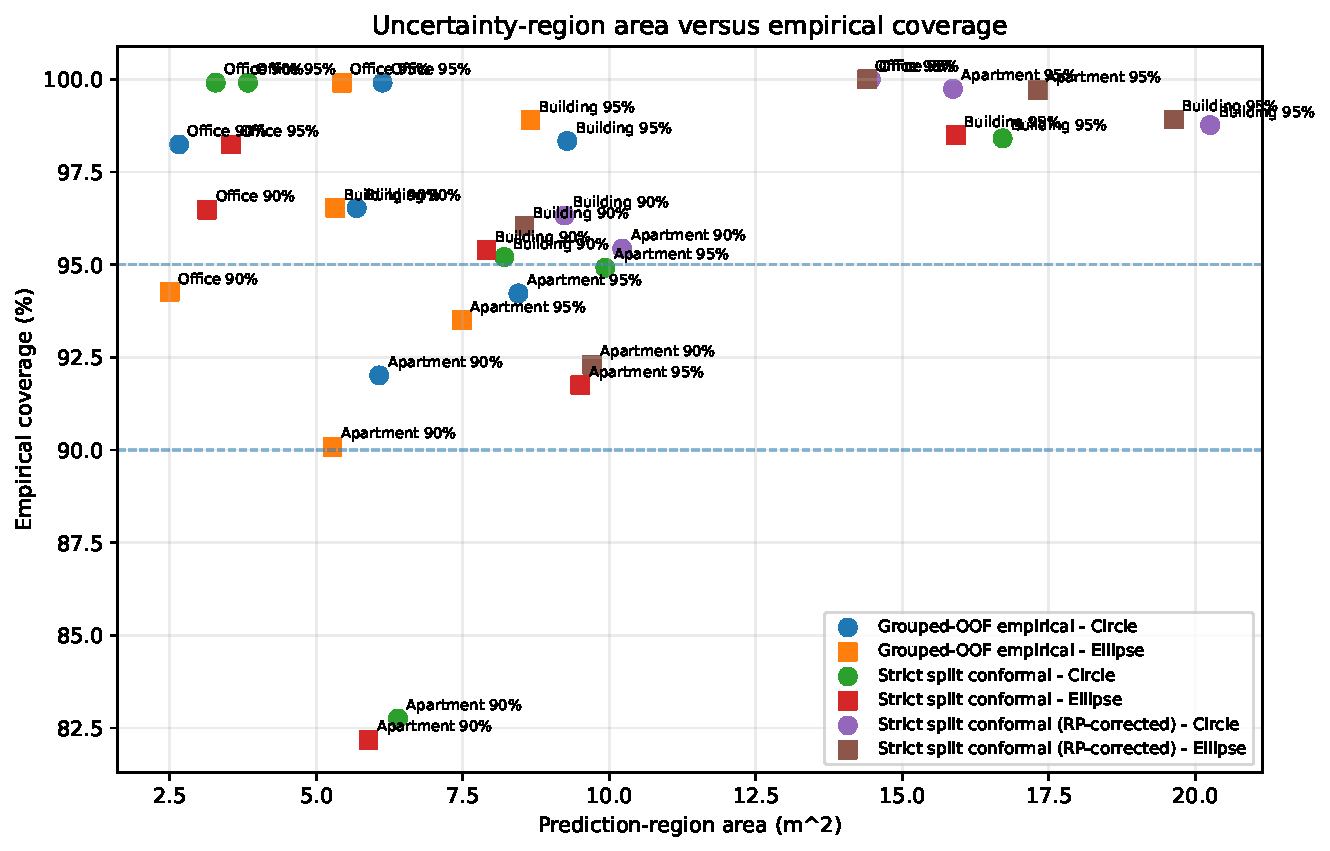
\includegraphics[width=0.8\textwidth]{fig12_uncertainty_area_coverage.pdf}
	\caption{Prediction-region area versus empirical coverage for circular and covariance-aware elliptical regions in a single calibration split (seed 42; values in Table~\ref{tab:s_uncertainty}).}
	\label{fig:s_uncertainty_area}
\end{figure}

\begin{figure}[!ht]
	\centering
	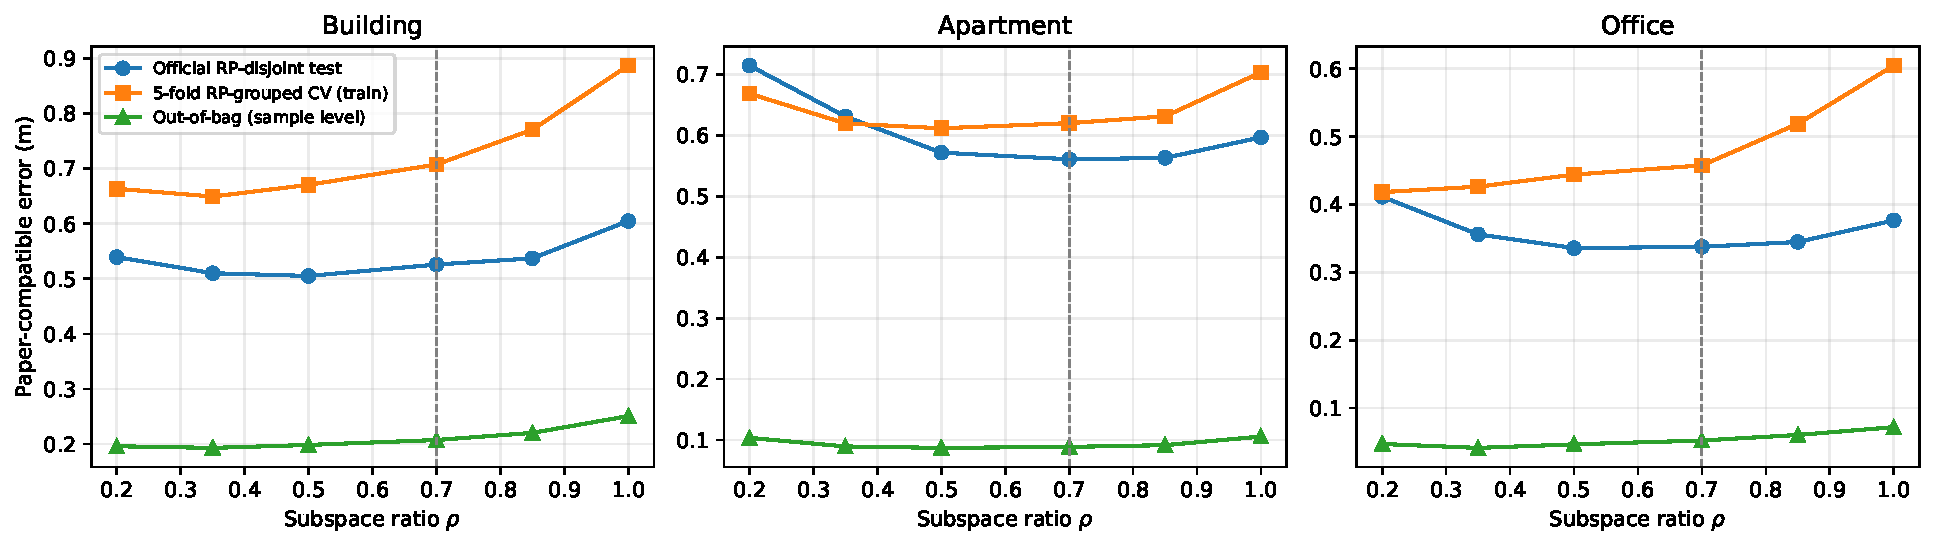
\includegraphics[width=\textwidth]{fig14_ratio_selection.pdf}
	\caption{Error versus subspace ratio as seen by the official RP-disjoint test, five-fold RP-grouped CV on the training RPs, and the out-of-bag error. The dashed line marks the fixed default $\rho=0.7$ (regret of each selection rule in the ratio-selection table of the paper).}
	\label{fig:s_ratio_selection}
\end{figure}


\begin{thebibliography}{1}
\bibitem{ho1998random}
T.~K. Ho, ``The random subspace method for constructing decision forests,'' \emph{IEEE Trans. Pattern Anal. Mach. Intell.}, vol.~20, no.~8, pp.~832--844, 1998.
\end{thebibliography}

\end{document}
